\documentclass[12pt,ngerman]{dtk}

\usepackage[utf8]{inputenc}
\usepackage[T1]{fontenc}
\usepackage{booktabs}
\usepackage{babel}
\usepackage{graphicx}
\usepackage{csquotes}
\usepackage{xcolor}
\usepackage{pgfornament,eso-pic,calc}
\usepackage{listings}

\title{Ordnerrücken gestalten mit \texttt{ticket.sty}}
\Author{Uwe}{Ziegenhagen}{Köln}

\begin{document}
\maketitle

\begin{abstract}
In diesem Artikel möchte ich kurz vorstellen, wie man mit \texttt{ticket.sty} einfach Ordnerrücken und andere Etiketten gestalten kann.
\end{abstract}


\section{Das \texttt{ticket} Paket}

Das Paket \texttt{ticket.sty}  ist mein persönlicher Favorit, wenn es um die Erzeugung von Etiketten aller Art mit \LaTeX\ geht. Das Paket wurde von Thomas Emmel entwickelt, aktuell ist die Version 0.40d aus dem Jahr 2016.

Zur Definition der einzelnen Etiketten trägt man die notwendigen Angaben in eine TDF-Datei ein, TDF steht dabei für \enquote{Ticket Definition File}. In diese Datei kommen Angaben zum Layout des Bogens (vertikaler und horizontaler Offset, gegebenenfalls druckerspezifisch) und die Angaben zu den einzelnen Etiketten: wieviele Spalten und Zeilen auf dem Bogen, Dimensionen eines einzelnen Tickets. In diesem Artikel soll die Nutzung des Pakets anhand von Ordnerrücken gezeigt werden, das Beispiel lässt sich aber auf nahezu jede Art von Etiketten und Labels übertragen.

\section{Ordnerrücken gestalten}

Betrachten wir am den folgenden Quellcode, der drei Etiketten für breite Ordner auf einem DIN~A4 Blatt erzeugt.

\begin{lstlisting}[language={[LaTeX]TeX}]
\documentclass[landscape]{scrartcl}
\usepackage[T1]{fontenc}
\usepackage{graphicx}
\usepackage[sfdefault]{plex-sans}

\begin{filecontents}[overwrite]{Ordner.tdf}
\unitlength=1mm
\hoffset=10mm
\voffset=-15mm
\ticketNumbers{1}{3}
\ticketSize{190}{58} % Breite und Hoehe der Labels in mm
\ticketDistance{0}{0} % Abstand der Labels
\end{filecontents}

\usepackage[Ordner]{ticket}

 
\renewcommand{\ticketdefault}{}%
\makeatletter
\@boxedtrue % Rahmen um Ticket
\@emptycrossmarkfalse % Falzmarken
\@cutmarktrue % Schnittmarken
\makeatother
 
\newcommand{\myticket}[2]{
\ticket{%
\put(15,15){\scalebox{#1}{\bfseries #2}}
}}
 
\begin{document}
\myticket{7}{Ausbildung}
\myticket{7}{Steuern}
\myticket{12}{ADAC}
\end{document}
\end{lstlisting}

Als Dokumentenklasse wähle ich \texttt{scrartcl}, da hier A4 als Dokumentengröße bereits vorgegeben ist und das Querformat einfach per Klassenoption gesetzt werden kann. Das Rumhantieren mit den Optionen vom \texttt{geometry} Paket kann daher entfallen. Aus dem \texttt{graphicx} Paket benötigen wir den \texttt{\textbackslash scalebox} Befehl, um die Schriftgröße innerhalb eines Labels beliebig skalieren zu können, als Schriftart kommt die IBM Plex Sans zum Einsatz.

Um nur mit einer Datei arbeiten zu müssen und nicht mehreren für Ticket-Definition und dem eigentlichen \TeX-Dokument, lege ich die Ticketdefinition in eine \texttt{filecontents}-Umgebung. Die \enquote{overwrite} Option sorgt dabei dafür, dass die Datei beim Kompilieren stets überschrieben wird, selbst wenn sie bereits existiert.

Wir legen die einzelnen Tickets mit der Größe 190 x 58 Millimeter an, zwischen den einzelnen Tickets soll es weder horizontalen noch vertikalen Abstand geben. Es passen drei Tickets in einer Spalte auf eine Seite, die vertikalen und horizontalen Offsets spielen bei unserem Beispiel keine Rolle, da wir nicht auf fertige Etikettenbögen drucken und werden auf nicht völlig unpassende Werte gesetzt.

Im nächsten Schritt laden wir das \texttt{ticket}-Paket, als Option übergeben wir den Namen unserer vorher geschriebenen TDF-Datei. Mit dem \texttt{\textbackslash renewcommand} Befehl setzen wir das Design des Ticket-Hintergrunds zurück, an dieser Stelle könnte man auch beispielsweise Bilder einbetten, die dann auf jedem Etikett gesetzt werden. 

Über die Befehle innerhalb von \texttt{makeatletter} und \texttt{makeatother} definieren wir, dass unsere Etiketten a) von einem Rahmen umgeben sind, b) Schnittmarken gesetzt und c) Falzmarken nicht gesetzt werden. 

Als nächsten definieren wir uns mit dem \texttt{\textbackslash myticket} Befehl ein Kommando für die Erzeugung der individuellen Etiketten. Wir benötigen dabei zwei Parameter, zum einen 
den Skalierungsfaktor für die Schriftgröße, zum anderen den Text, der auf das jeweilige Etikett gesetzt werden soll. 

In das eigentliche Dokument kommen dann nur noch die \texttt{\textbackslash myticket} Befehle mit den jeweiligen Parametern für Textskalierung und Inhalt.

Gesetzt sieht das Ganze dann so aus wie in der folgenden Abbildung dargestellt.

\fbox{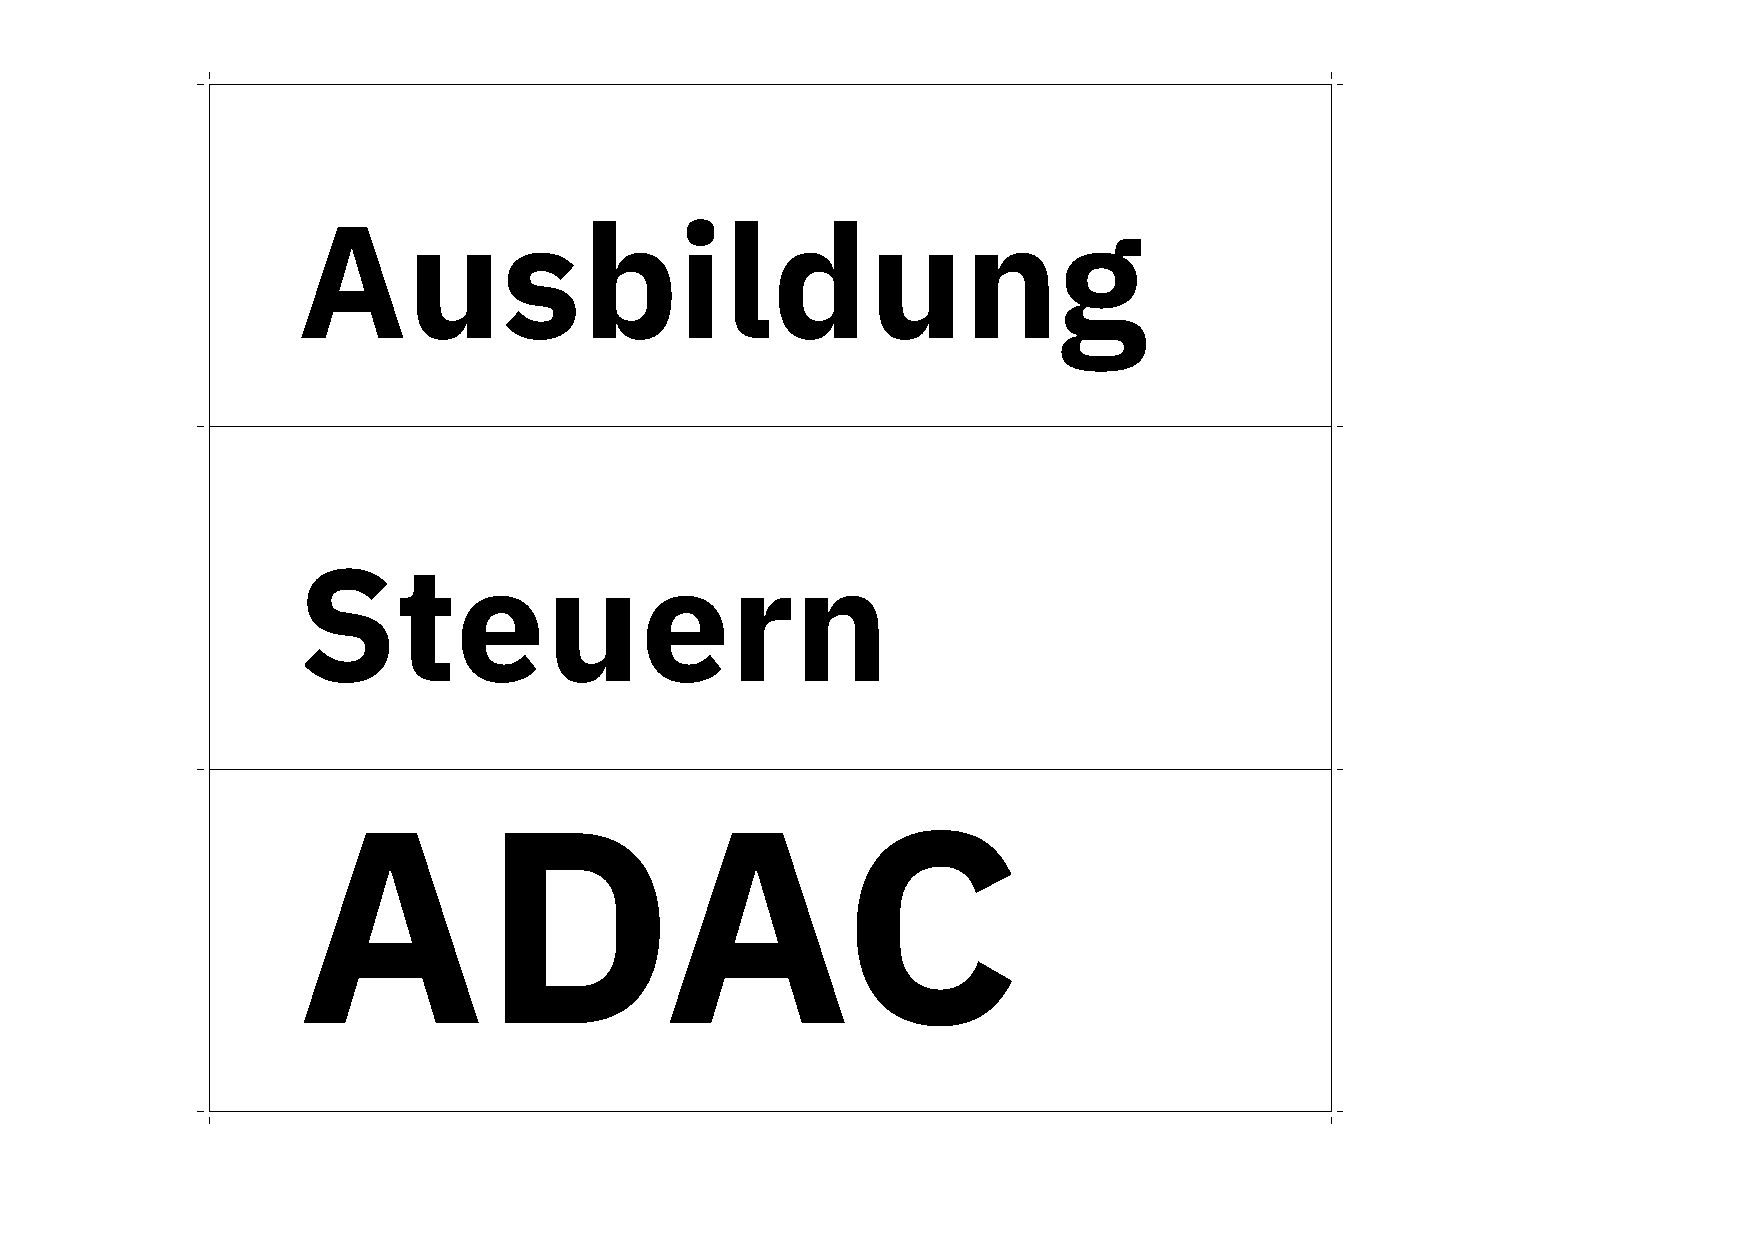
\includegraphics[width=\textwidth]{OrdnerBeispiel}}

\section{Fazit}

Mit \texttt{ticket.sty} lassen sich in kurzer Zeit Etiketten und Labels jeder Art gestalten. Eine TDF-Datei ist schnell geschrieben, die Einbettung der Definition in den \TeX-Code sorgt dafür, dass man stets nur eine Datei bearbeiten muss. 

\end{document}